\documentclass[11pt, a4paper]{article}
%\usepackage{proj1}
\usepackage{natbib}
\usepackage{fancyhdr}  
\usepackage{subcaption}
\usepackage{caption}
\usepackage{graphicx}
\usepackage{numprint}
\usepackage{multirow}
\linespread{1.25} 
\setlength{\parindent}{0cm}
\graphicspath{{Images/}}
\usepackage{hyperref}
\usepackage{amsmath}
\usepackage{amsfonts}
\usepackage{amssymb}
\usepackage{amsthm}
\usepackage{mathtools}
\usepackage{commath}
\usepackage{bbm}

%\usepackage[sc,osf]{mathpazo}
\usepackage{subcaption}
\usepackage[a4paper, top=1in, left=1.0in, right=1.0in, bottom=1in, includehead, includefoot]{geometry} %Usually have top as 1in

\usepackage{listings}
\usepackage{color} %red, green, blue, yellow, cyan, magenta, black, white
\definecolor{mygreen}{RGB}{28,172,0} % color values Red, Green, Blue
\definecolor{mylilas}{RGB}{170,55,241}


\hypersetup{colorlinks,linkcolor={black},citecolor={blue},urlcolor={black}}
\usepackage{color}
\urlstyle{same}


\theoremstyle{definition}
\newtheorem{definition}{Definition}[section]

%\newcommand{\Sta}{\rho}
\newcommand{\Adj}{p}
\newcommand{\adj}{q}
%\newcommand{\Con}{u}
\newcommand{\Sta}{\rho}
\newcommand{\Stav}{\mathbf{v}}
\newcommand{\Adja}{\mathbf{p}}
\newcommand{\Adjb}{q}
\newcommand{\Adjc}{{p}_{\partial \Sigma}}
\newcommand{\Con}{\mathbf{f}}
\newcommand{\nor}{\mathbf{n}}




\pagenumbering{gobble}
\begin{document}
	\section*{Report 13/08/2020}
	\section{Rewriting 1D Input of Interaction Kernel}
	Changed input of interaction kernel from $\nabla V_2$ to $V_2$. Took the below example (Example 2 from paper) to compare.
	The cost functionals are the same.
	The results of the optimization are within the tolerances:
	\begin{align*}
		\rho_{Diff} = 6.2060 \times 10^{-9} \quad q_{Diff} = 1.1993 \times 10^{-10} \quad \vec w_{Diff} = 9.8629 \times 10^{-8},
	\end{align*}
	as measured by the L2Linfinity norm. 
\section{Moving External Potentials}
We consider Example 2 from the paper:
\begin{equation*}
\widehat \rho = \frac{1-t}{2}\left(\cos(\pi x) + 1 \right) + \frac{t}{2}\left(-\cos(2 \pi x) + 1 \right), \ \
\rho_{0} = \frac{1}{2}\cos(\pi x) + \frac{1}{2},\ \
f =0,\ \
V_{ext} =0,
\end{equation*}
and changing $V_{ext}$ in different, time dependent, ways. The number of points for the examples $N=30$, $n=20$, the tolerances are $10^{-8}/10^{-4}$, $\beta = 10^{-3}$.
The baseline example has the following results:
For $\kappa = -1$, $J_{FW} = 0.0536$, $J_{Opt} = 0.0096$, see Figure \ref{F0}.
For $\kappa = 1$, $J_{FW} = 0.0839$, $J_{Opt} = 0.0125$, see Figure \ref{F0a}.


\begin{figure}[h]
	\centering
	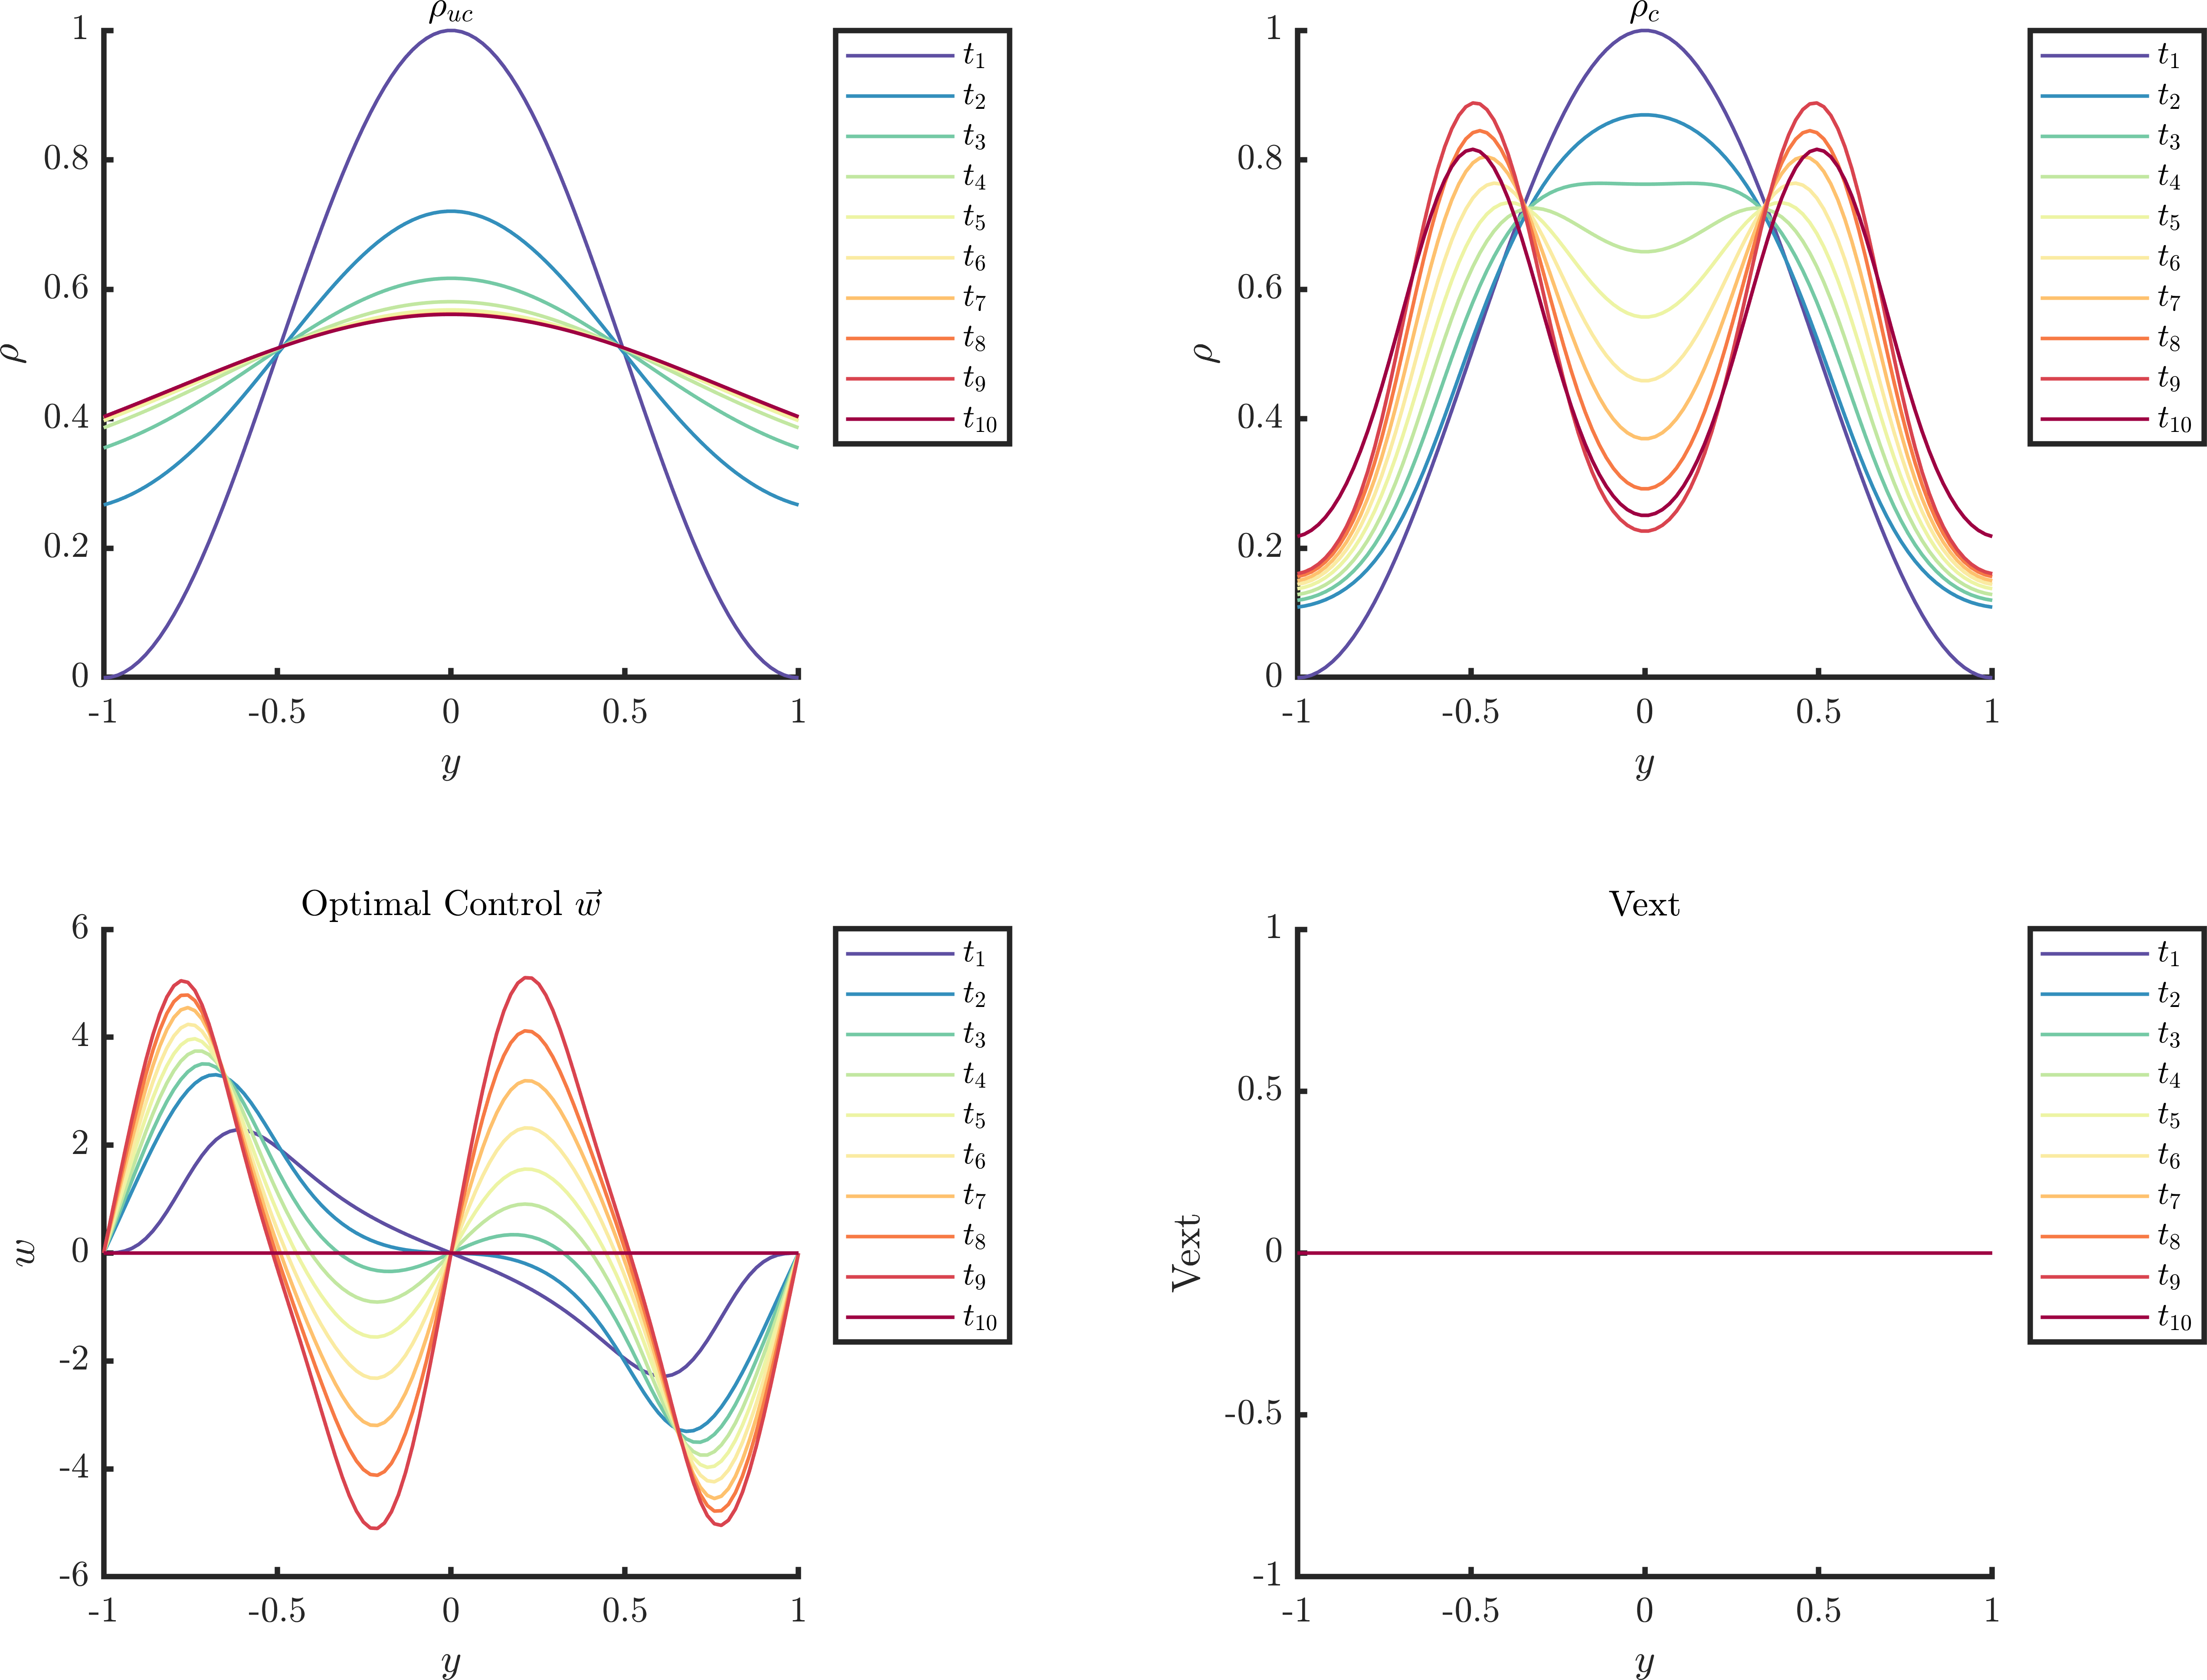
\includegraphics[scale=0.055]{Vext0n1.png}
	\caption{$V_{ext0}$, $\kappa = -1$} 
	\label{F0}
\end{figure}
\begin{figure}[h]
	\centering
	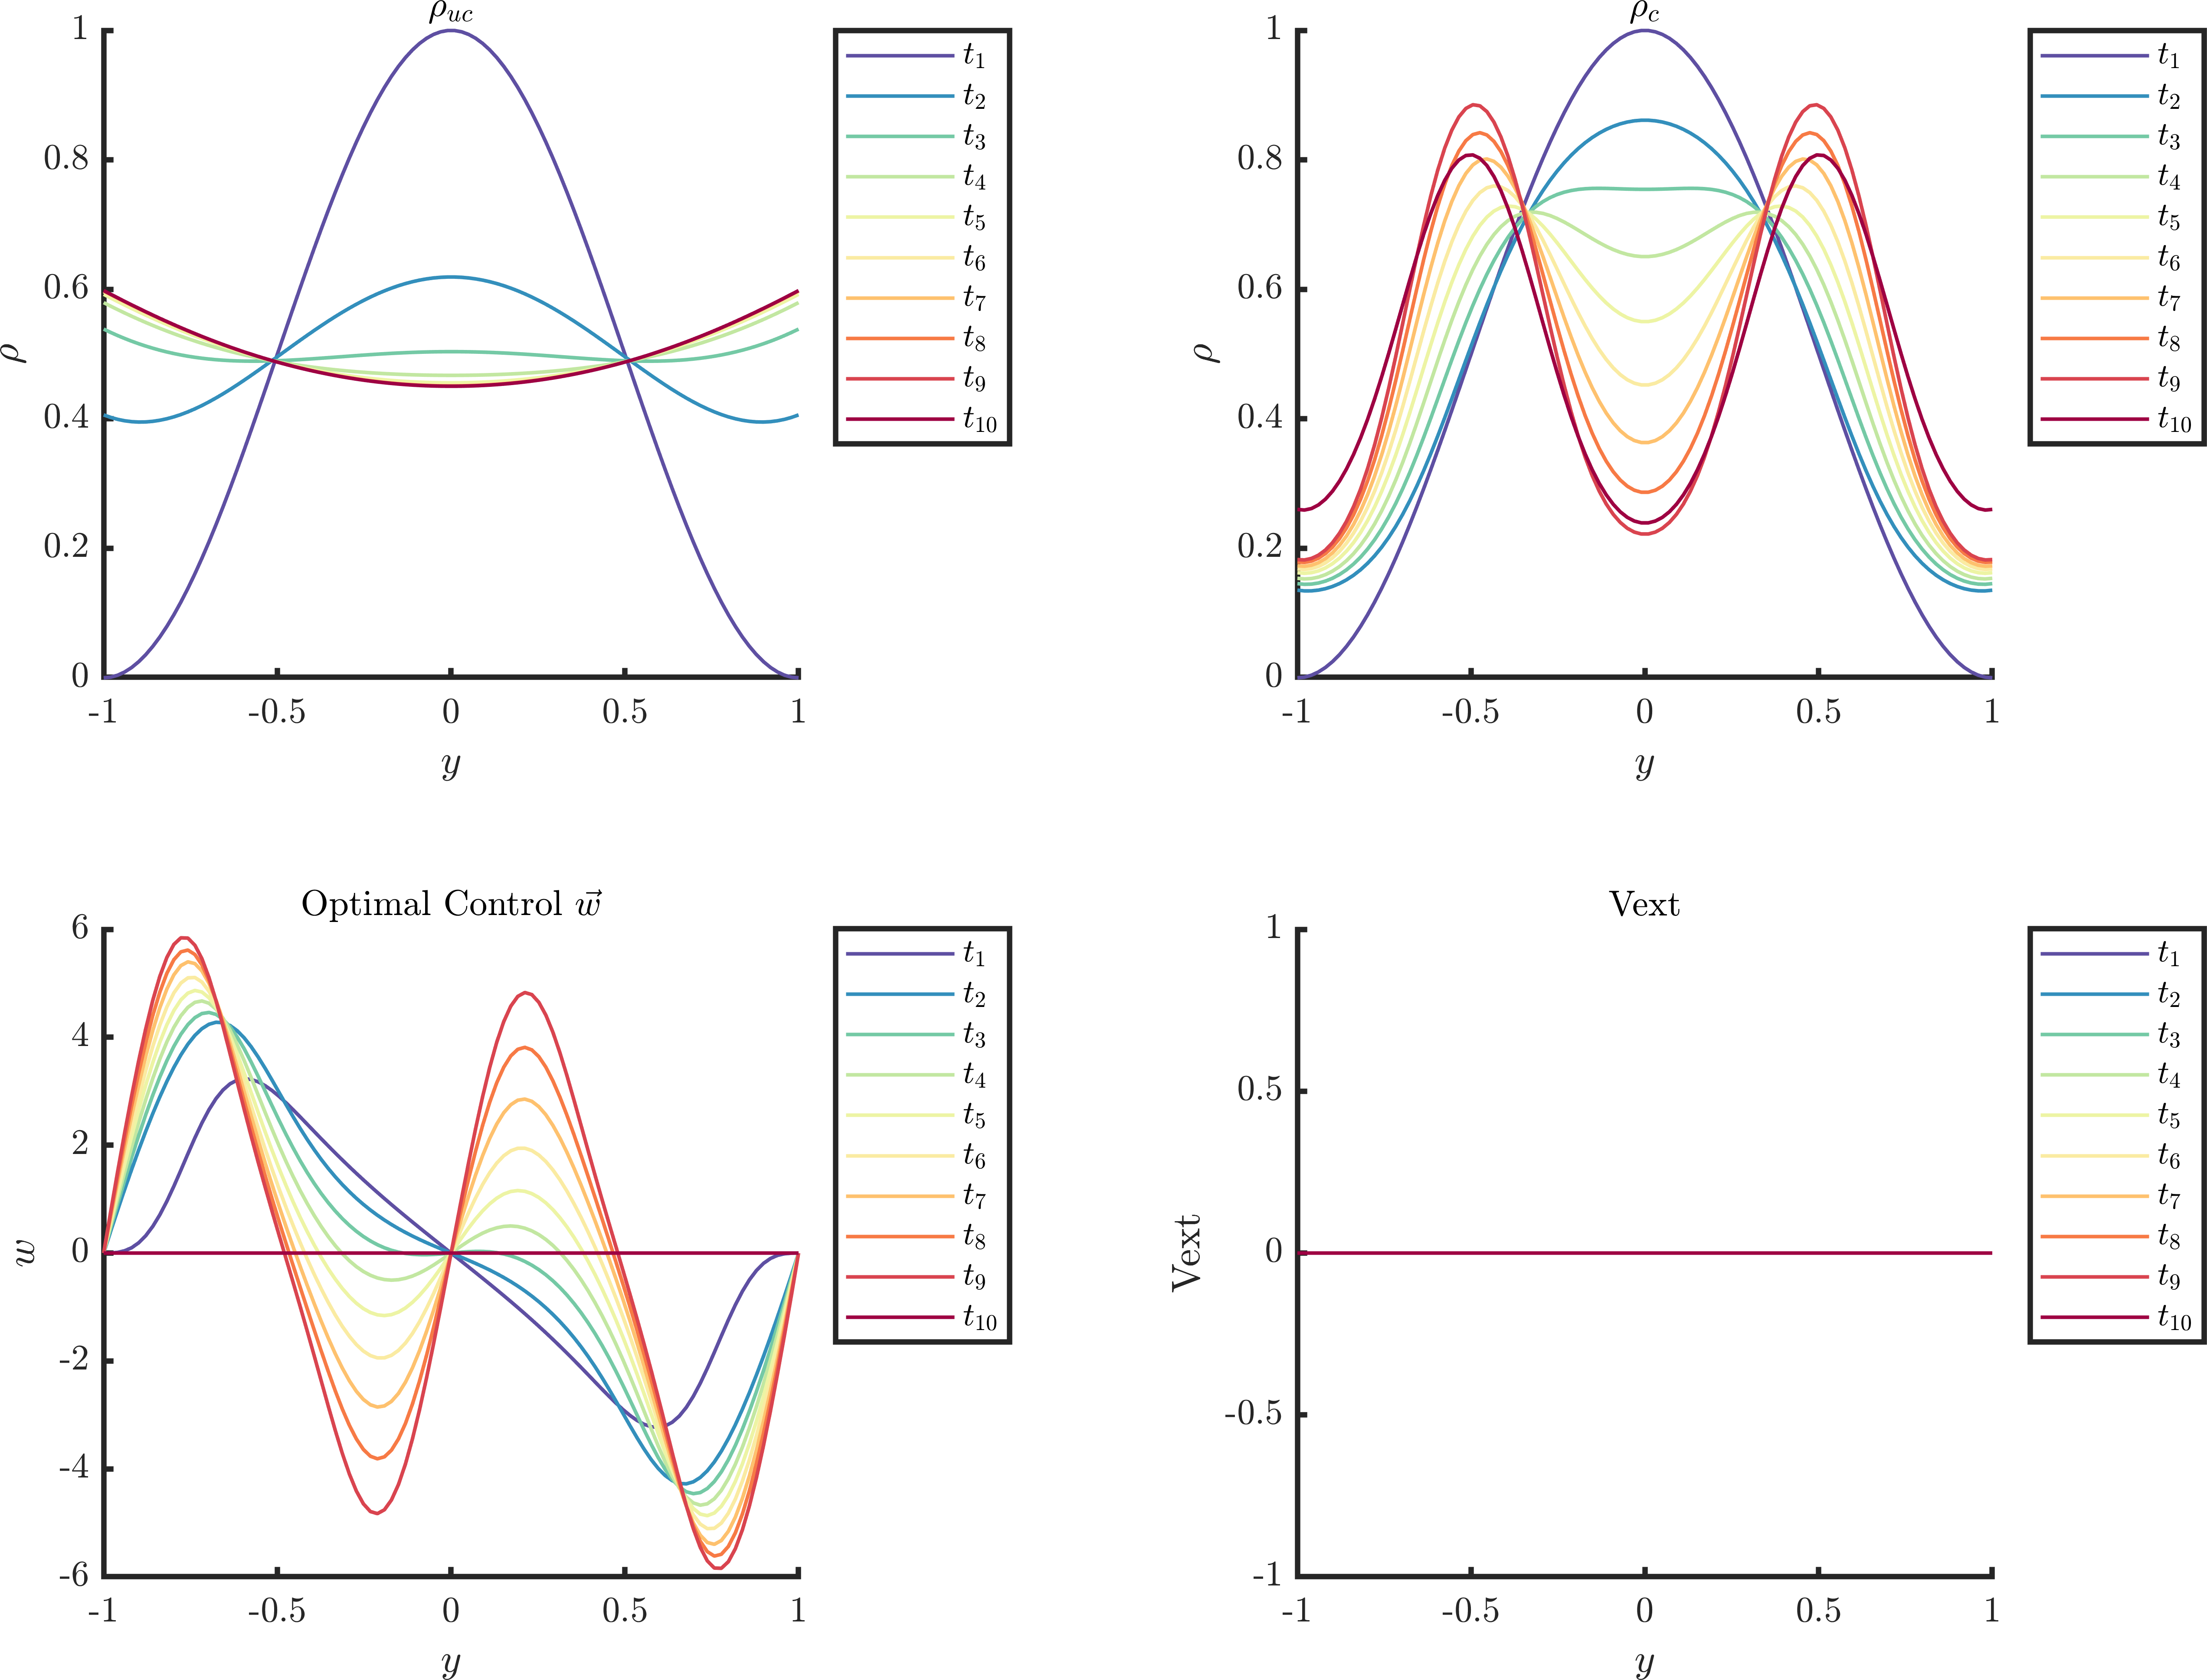
\includegraphics[scale=0.055]{Vext01.png}
	\caption{$V_{ext0}$, $\kappa = 1$} 
	\label{F0a}
\end{figure}
First example:
\begin{align*}
V_{ext} = t\cos(\pi y).
\end{align*}
For $\kappa = -1$, $J_{FW} = 0.1112$, $J_{Opt} = 0.0119$, see Figure \ref{F1}.
For $\kappa = 1$, $J_{FW} = 0.1612$, $J_{Opt} = 0.0161$, see Figure \ref{F1a}.


\begin{figure}[h]
	\centering
	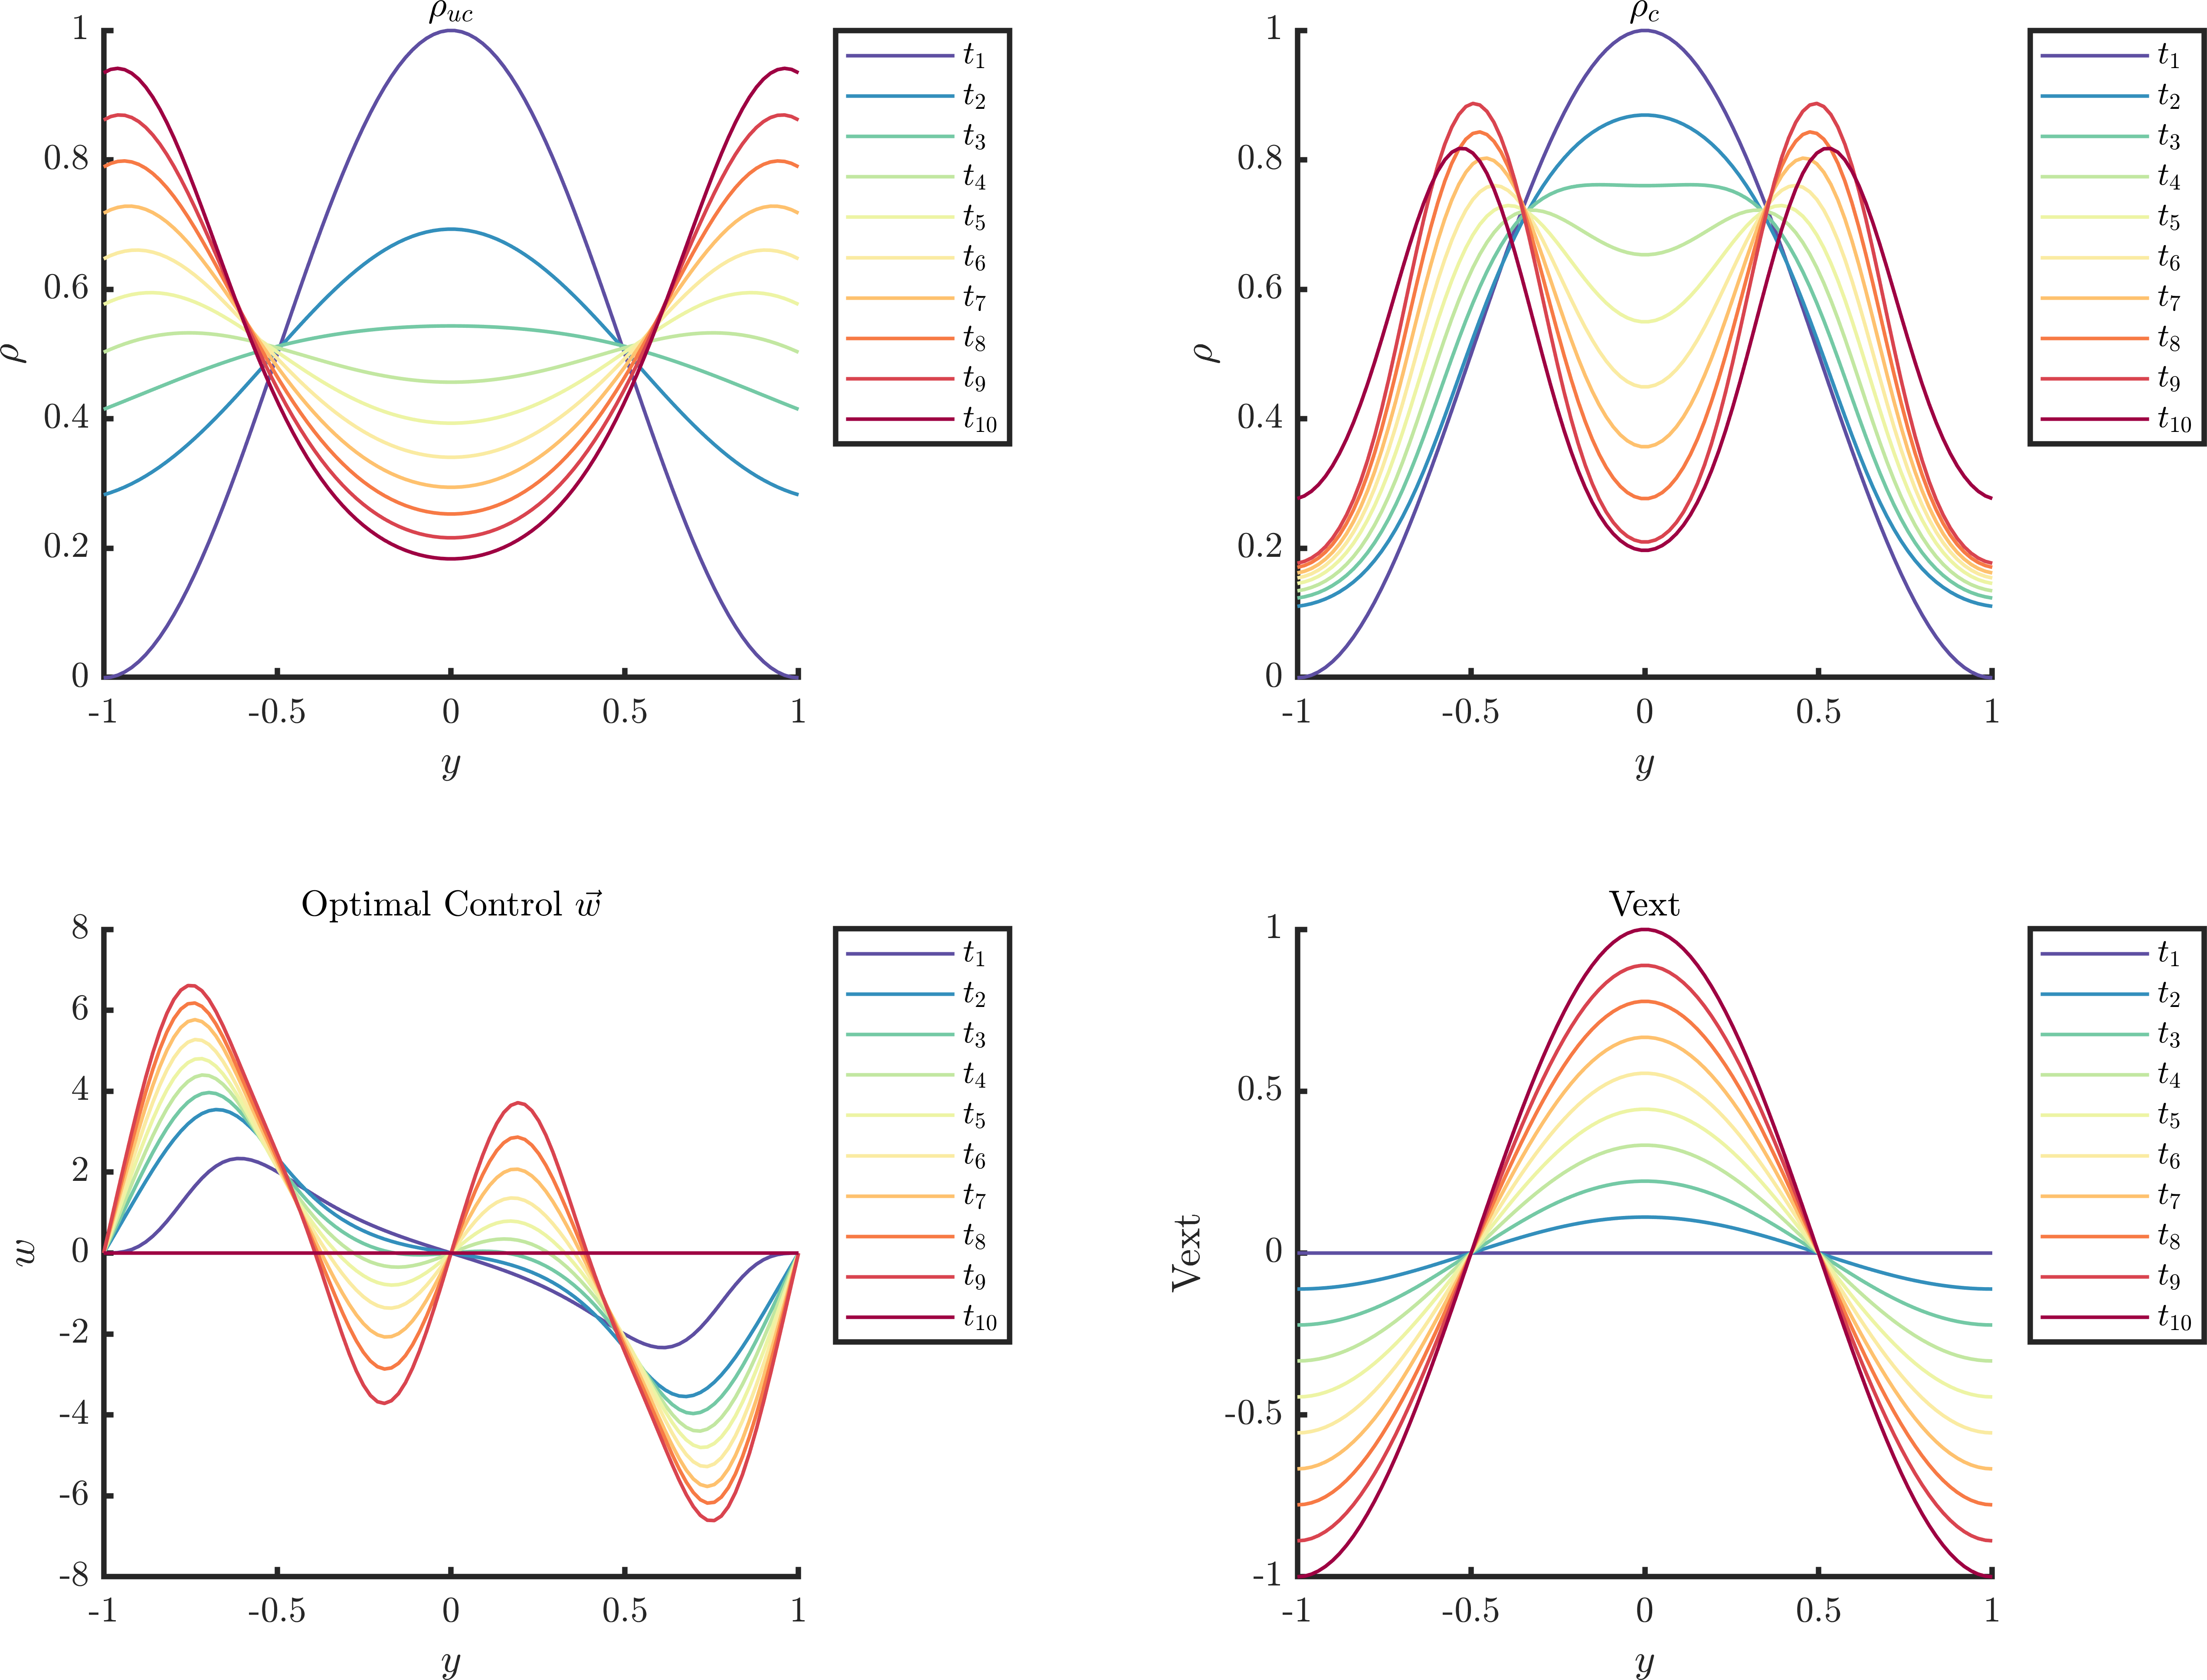
\includegraphics[scale=0.055]{Vext1n1.png}
	\caption{$V_{ext1}$, $\kappa = -1$} 
	\label{F1}
\end{figure}
\begin{figure}[h]
	\centering
	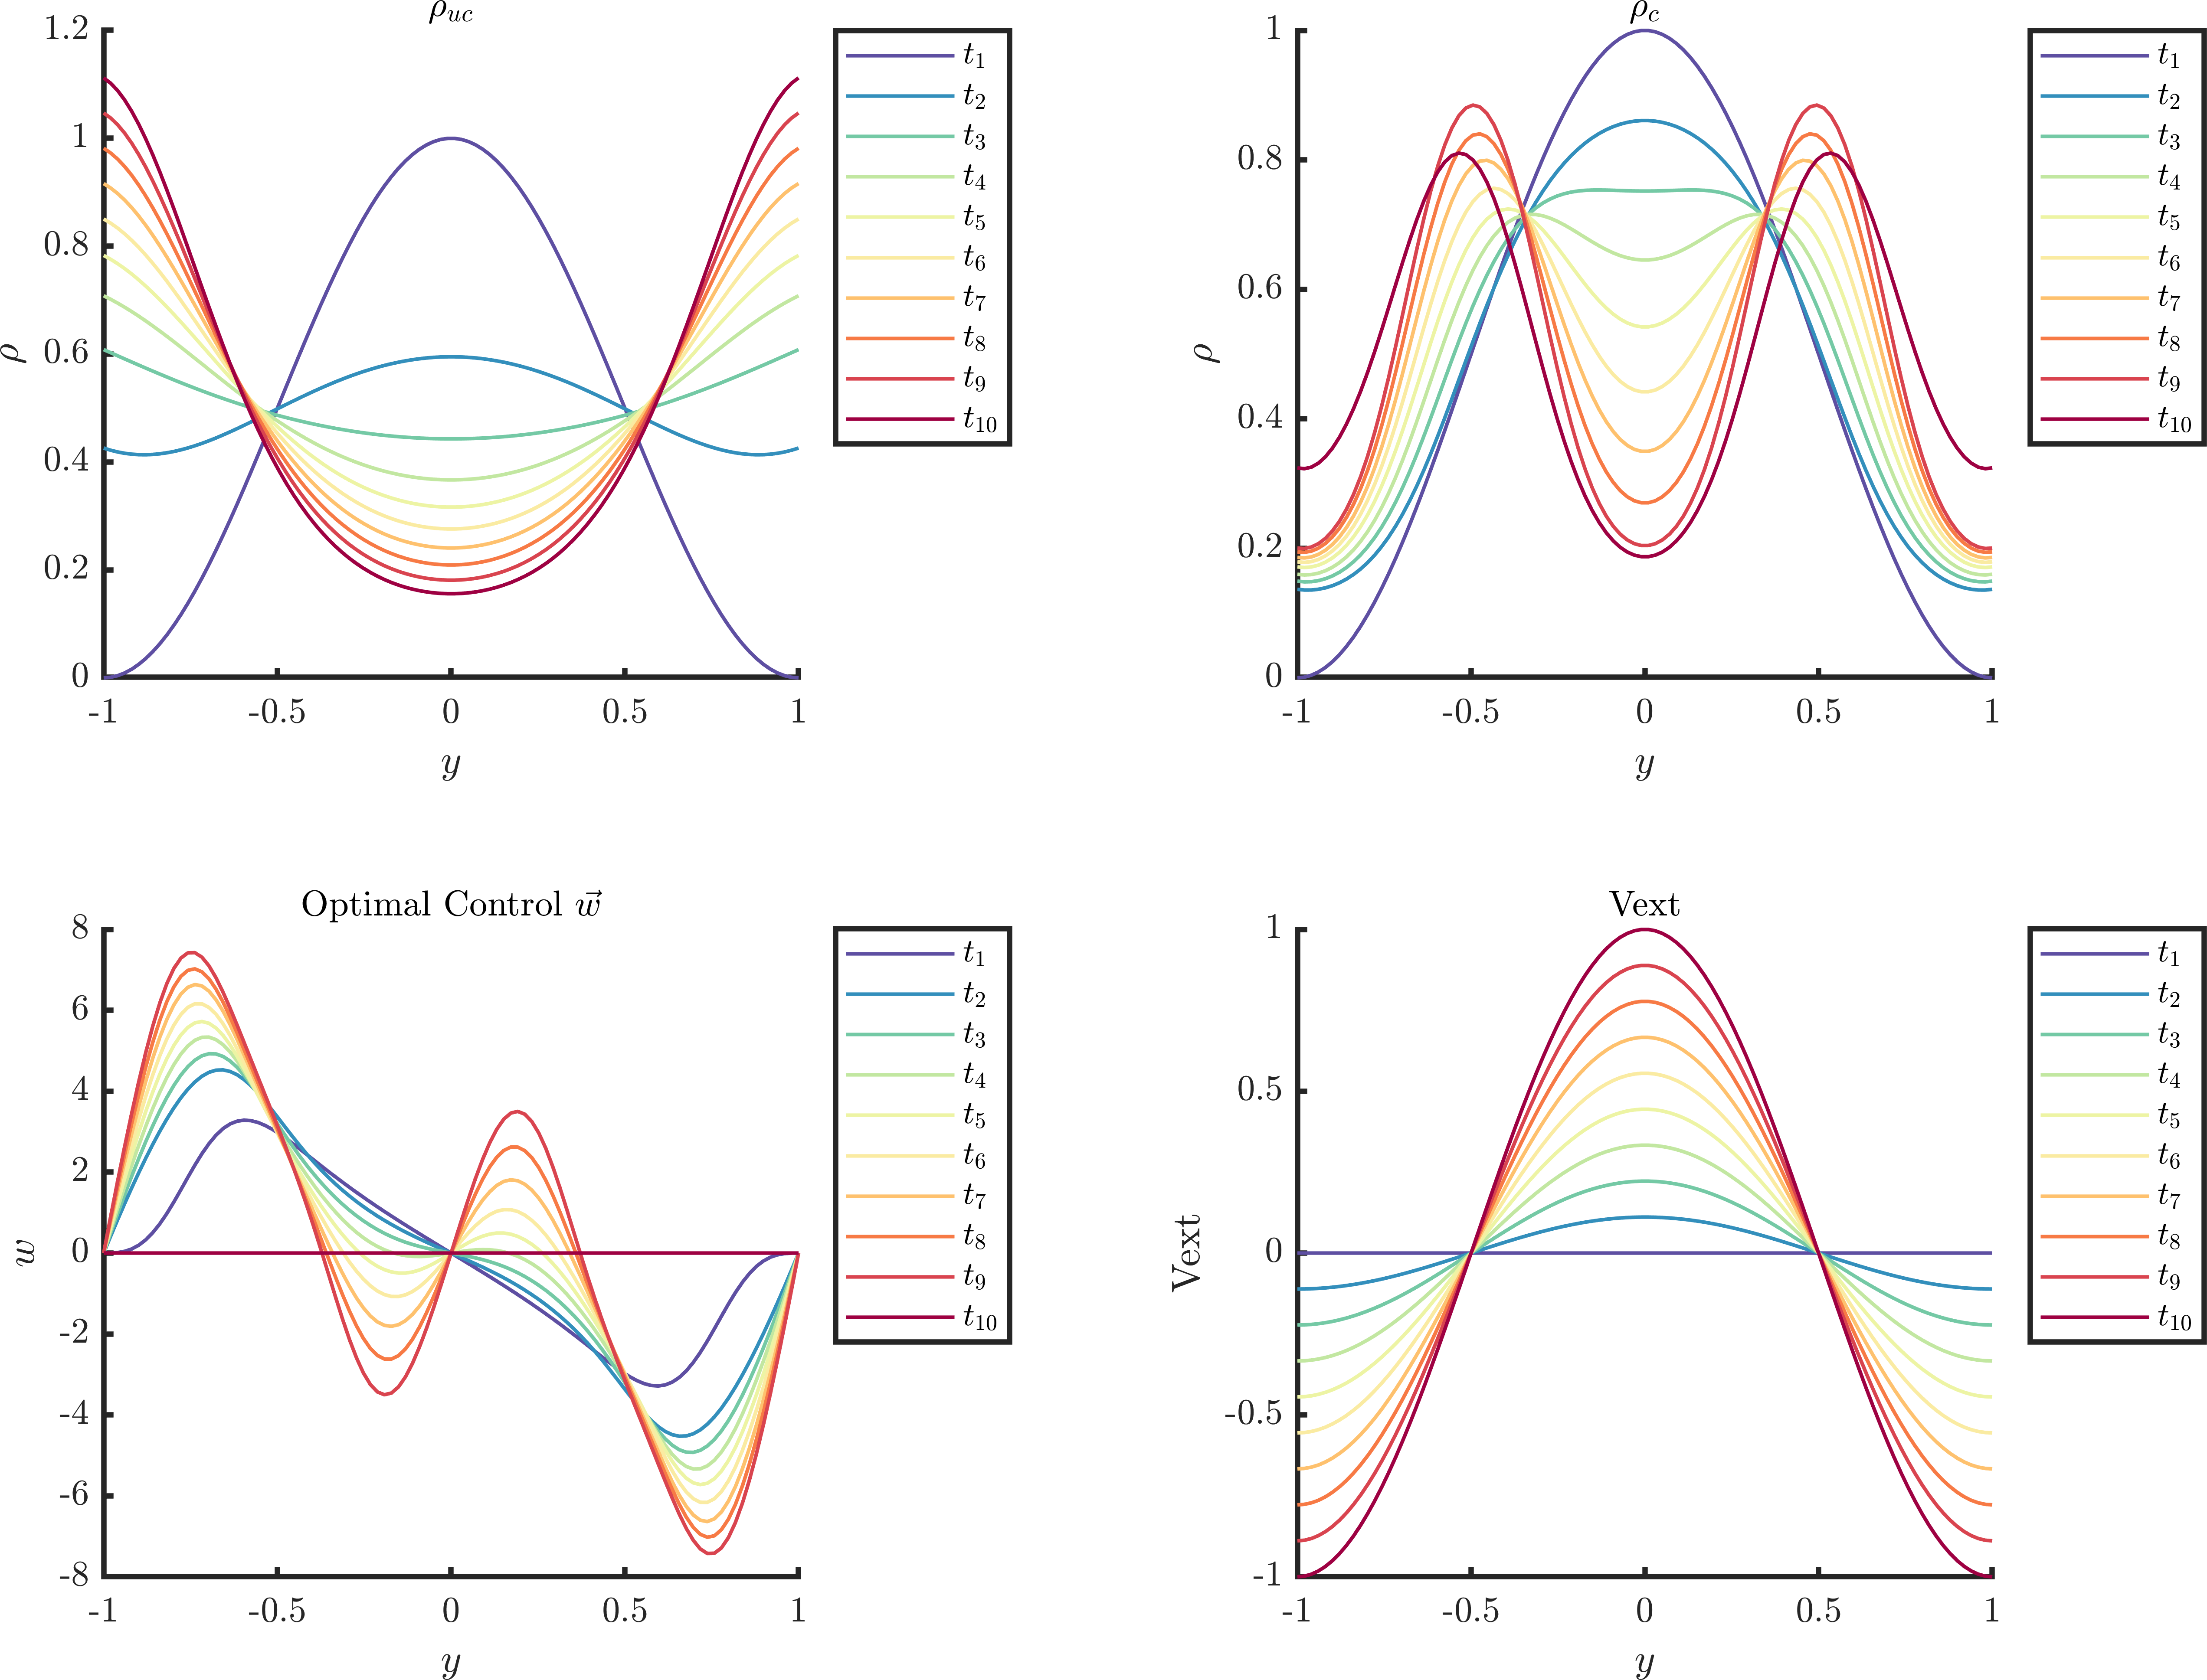
\includegraphics[scale=0.055]{Vext11.png}
	\caption{$V_{ext1}$, $\kappa = 1$} 
	\label{F1a}
\end{figure}

Second example:
\begin{align*}
V_{ext} = (1-t)\sin(\pi y) + t\cos(\pi y).
\end{align*}
For $\kappa = -1$, $J_{FW} = 0.1601$, $J_{Opt} = 0.0131$, see Figure \ref{F2}.
For $\kappa = 1$, $J_{FW} = 0.1822$, $J_{Opt} = 0.0173$, see Figure \ref{F2a}.


\begin{figure}[h]
	\centering
	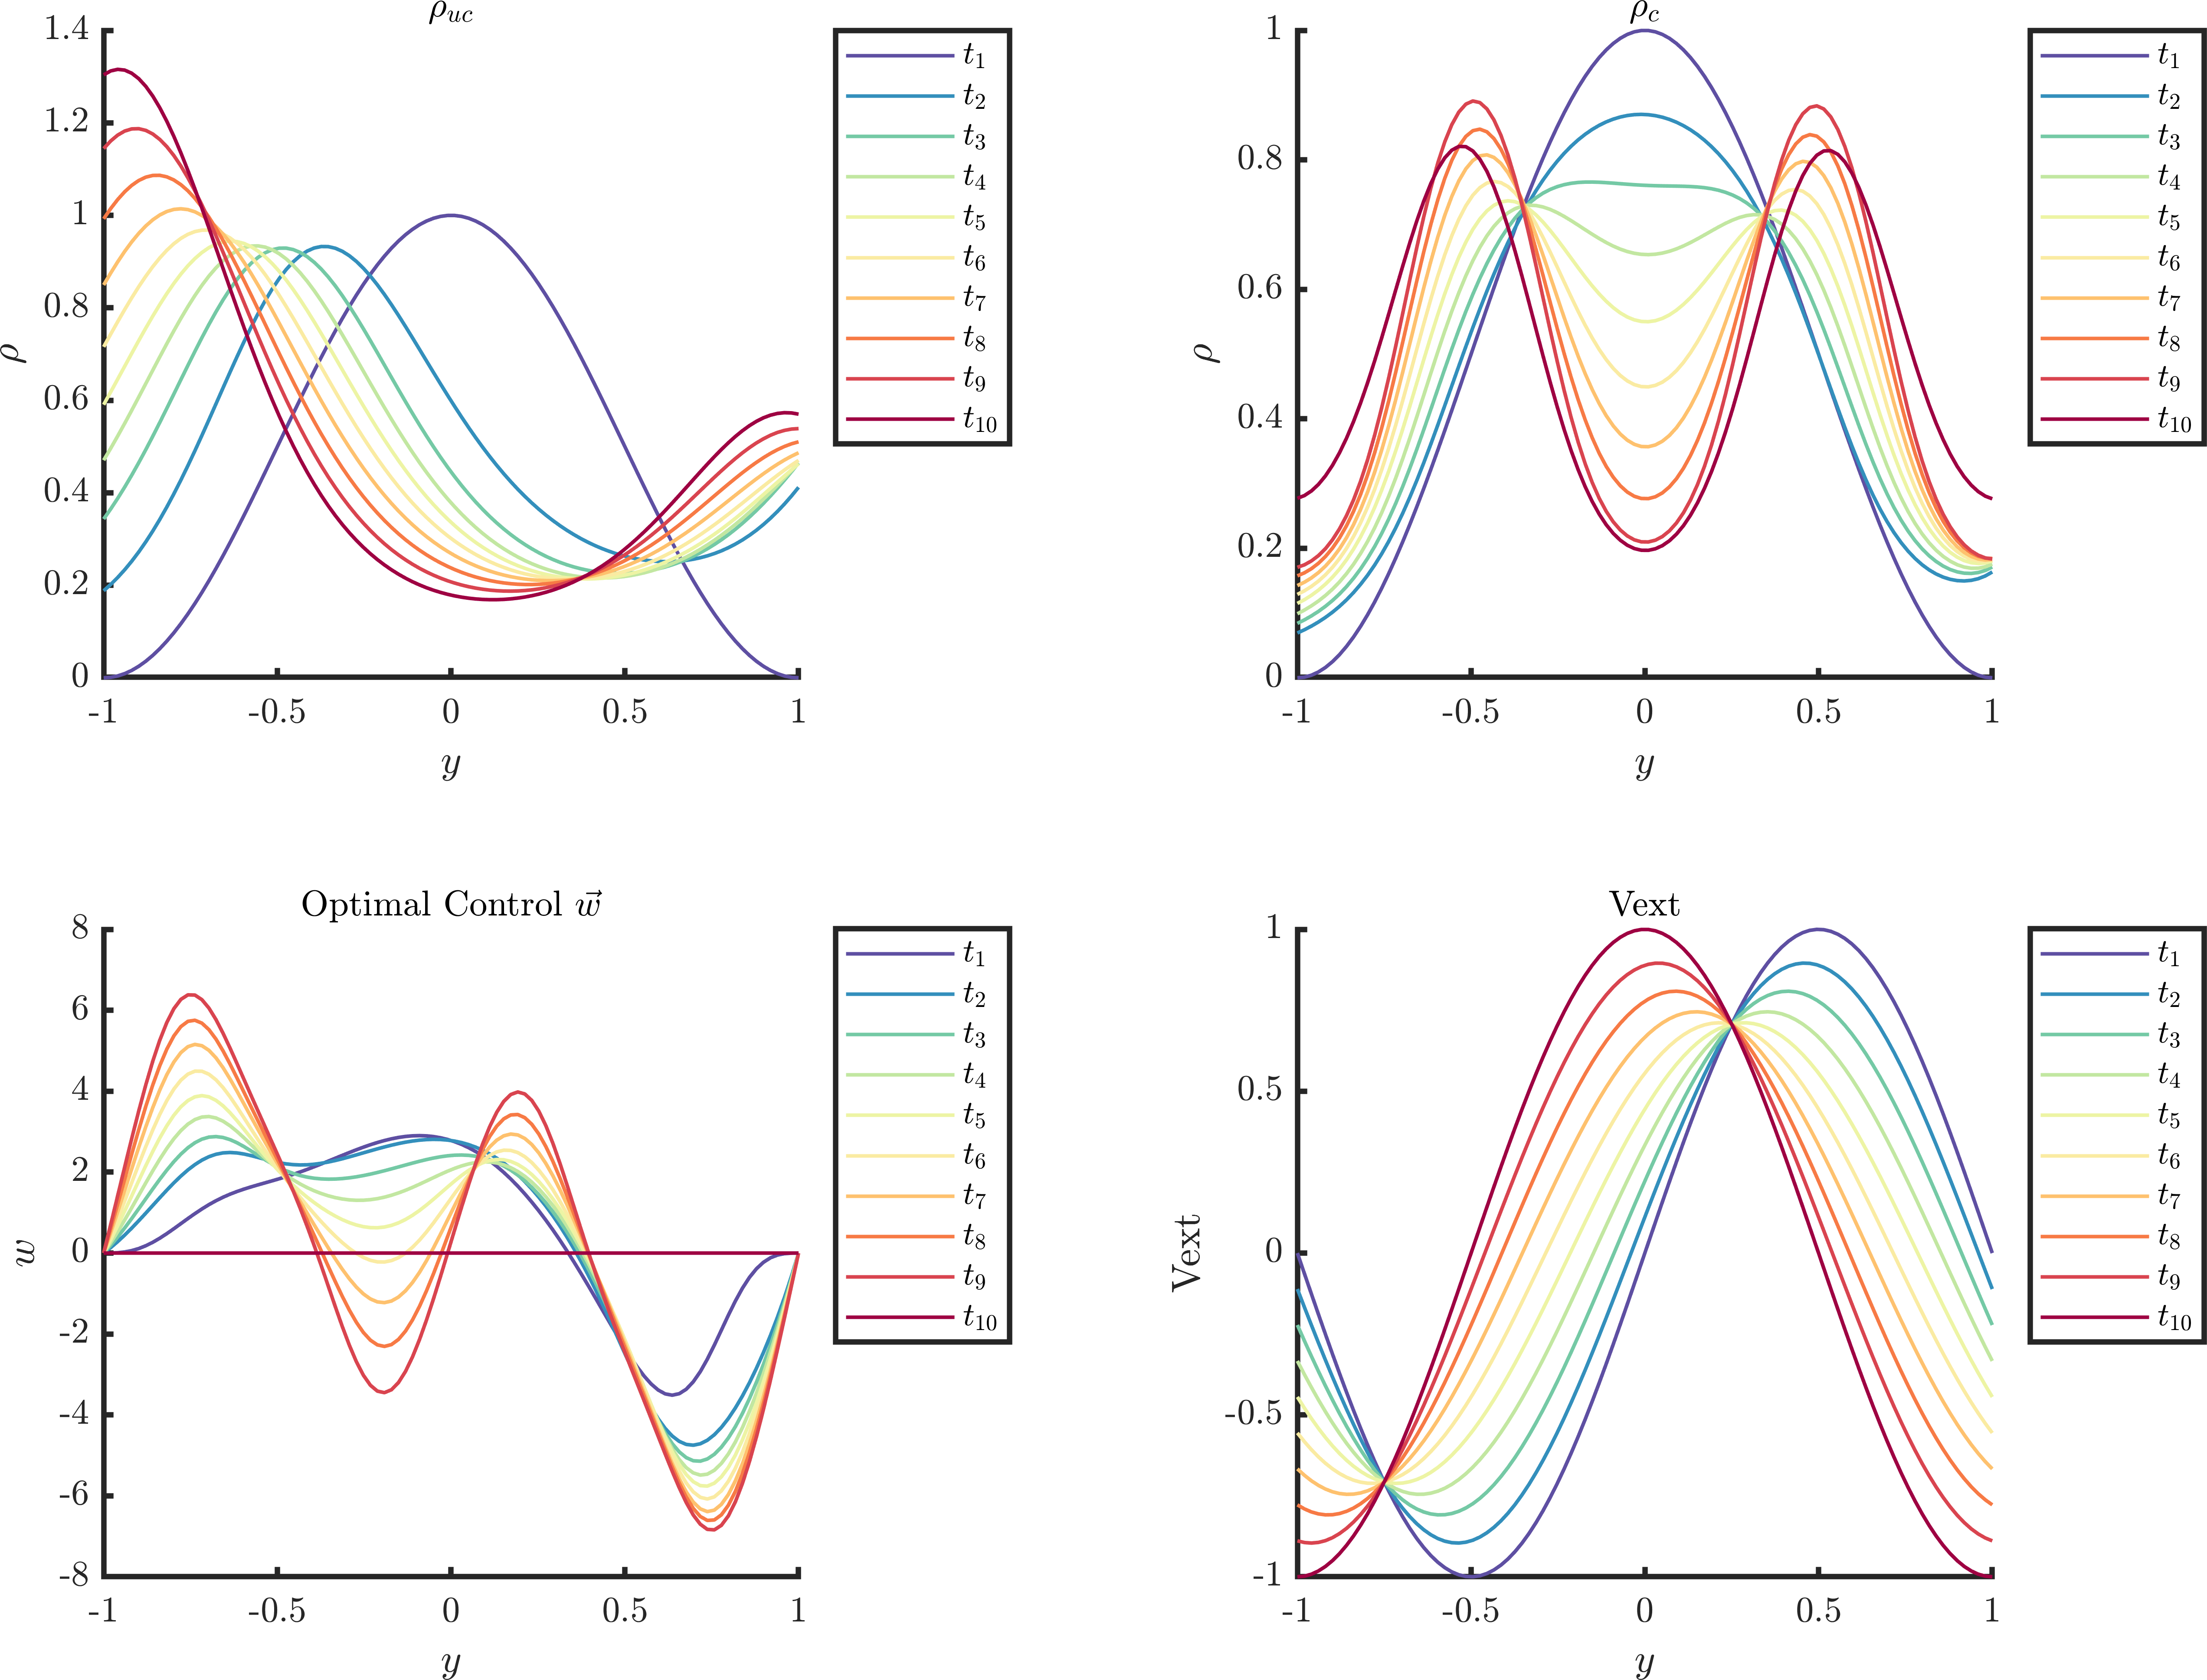
\includegraphics[scale=0.055]{Vext2n1.png}
	\caption{$V_{ext2}$, $\kappa = -1$} 
	\label{F2}
\end{figure}
\begin{figure}[h]
	\centering
	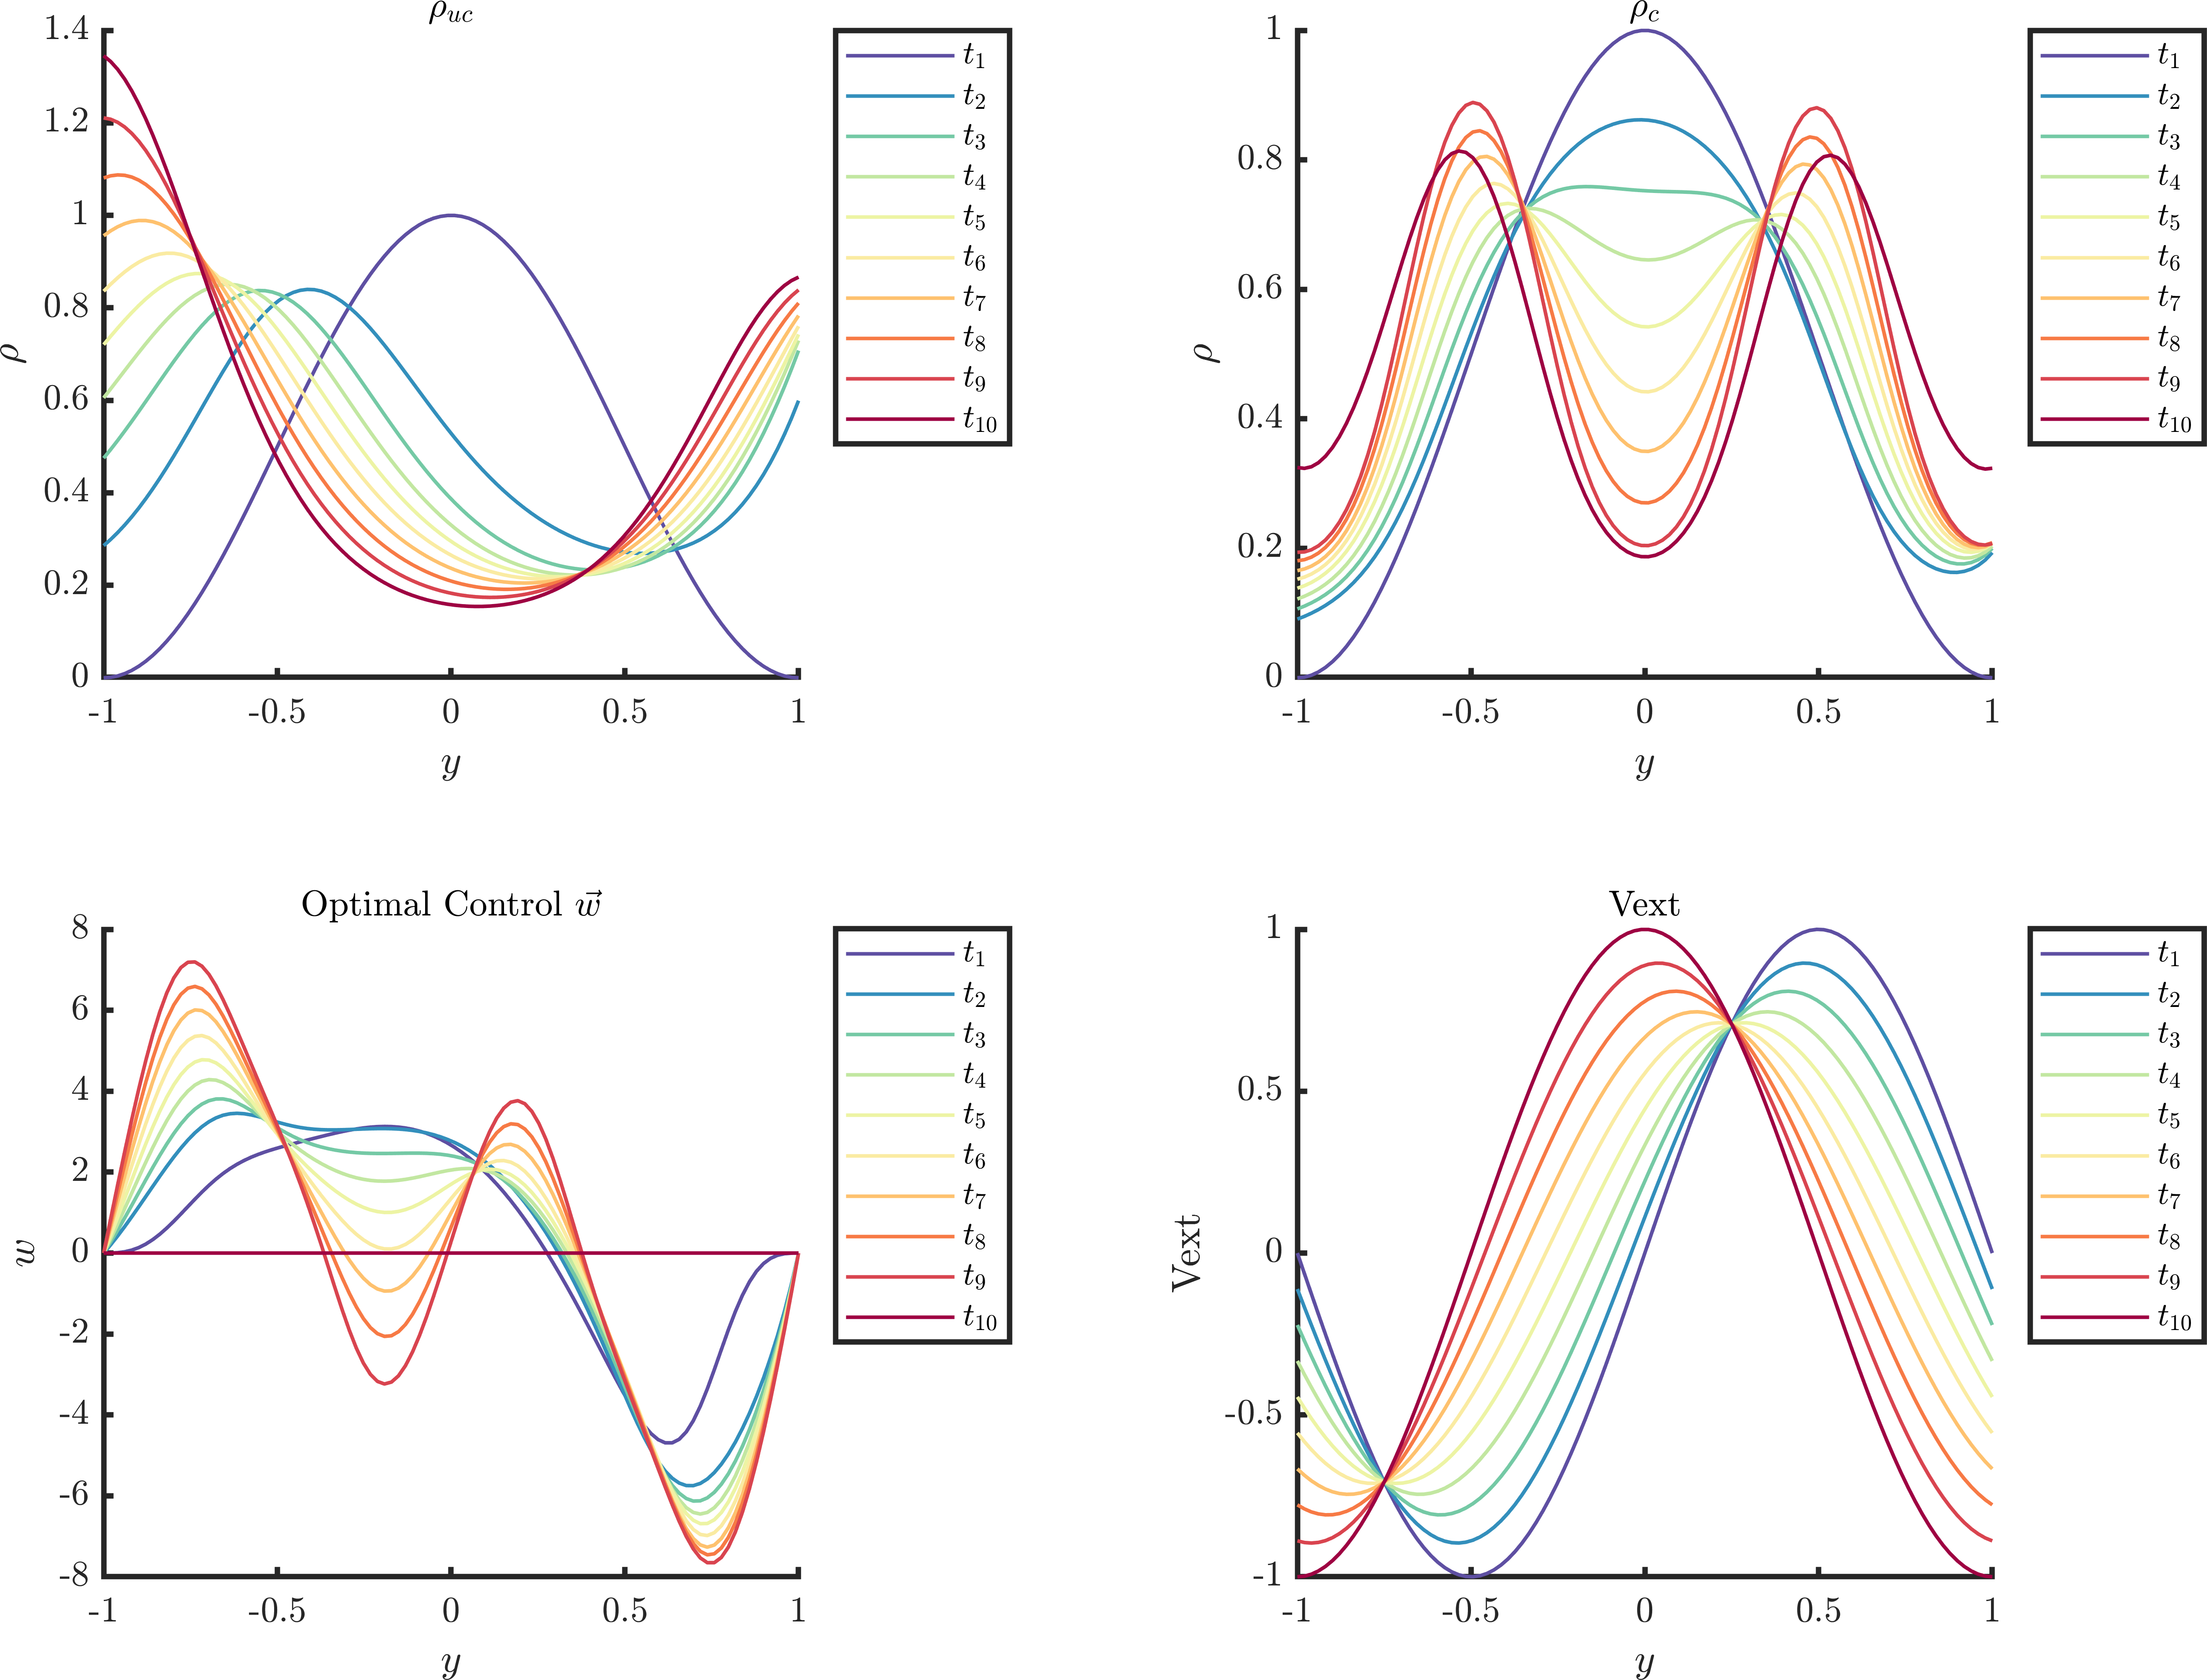
\includegraphics[scale=0.055]{Vext21.png}
	\caption{$V_{ext2}$, $\kappa = 1$} 
	\label{F2a}
\end{figure}

We can see overall when comparing to the case without any external potential, that the forward problem is changed quite drastically depending on the potential. Equally impacted is the optimal control. 
The difference between attractive and repulsive cases can be seen on the boundary of the forward solution mostly.
Overall, applying the external potential makes the problem more costly, as can be seen by comparing the different $J_{FW}$. However, the control effect with $\beta = 10^{-3}$ is a change of order one in all of the examples.


\section{Changing $V_2$}
We consider again:\\
\begin{equation*}
\widehat \rho = \frac{1-t}{2}\left(\cos(\pi x) + 1 \right) + \frac{t}{2}\left(-\cos(2 \pi x) + 1 \right), \ \
\rho_{0} = \frac{1}{2}\cos(\pi x) + \frac{1}{2},\ \
f =0,\ \
V_{ext} =0,
\end{equation*}
Number of points $N=40$, $n=30$, but for no good reason.
We now change $V_2$ from a Gaussian, to the following:
\begin{align*}
V_2 = e^{0.3(y-1)^2} + e^{-5(y-1)^2}.
\end{align*}
For $\kappa = -1$, $J_{FW} = 0.2241$, $J_{Opt} = 0.0186$, see Figure \ref{F3}.
For $\kappa = 1$, $J_{FW} = 0.1016$, $J_{Opt} = 0.0087$, see Figure \ref{F3a}.
\begin{figure}[h]
	\centering
	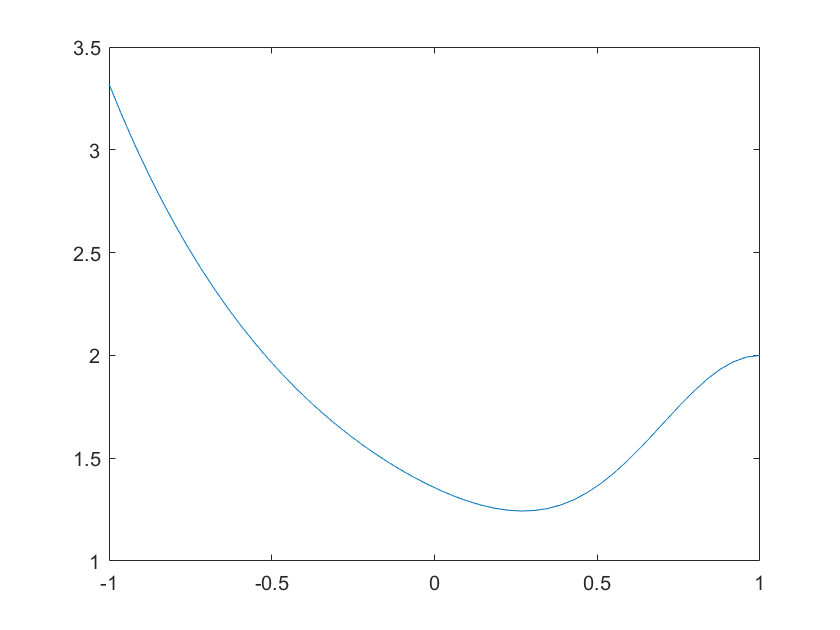
\includegraphics[scale=0.5]{V2.png}
	\caption{$V_{2}$, $\kappa = -1$} 
	\label{F30}
\end{figure}
\begin{figure}[h]
	\centering
	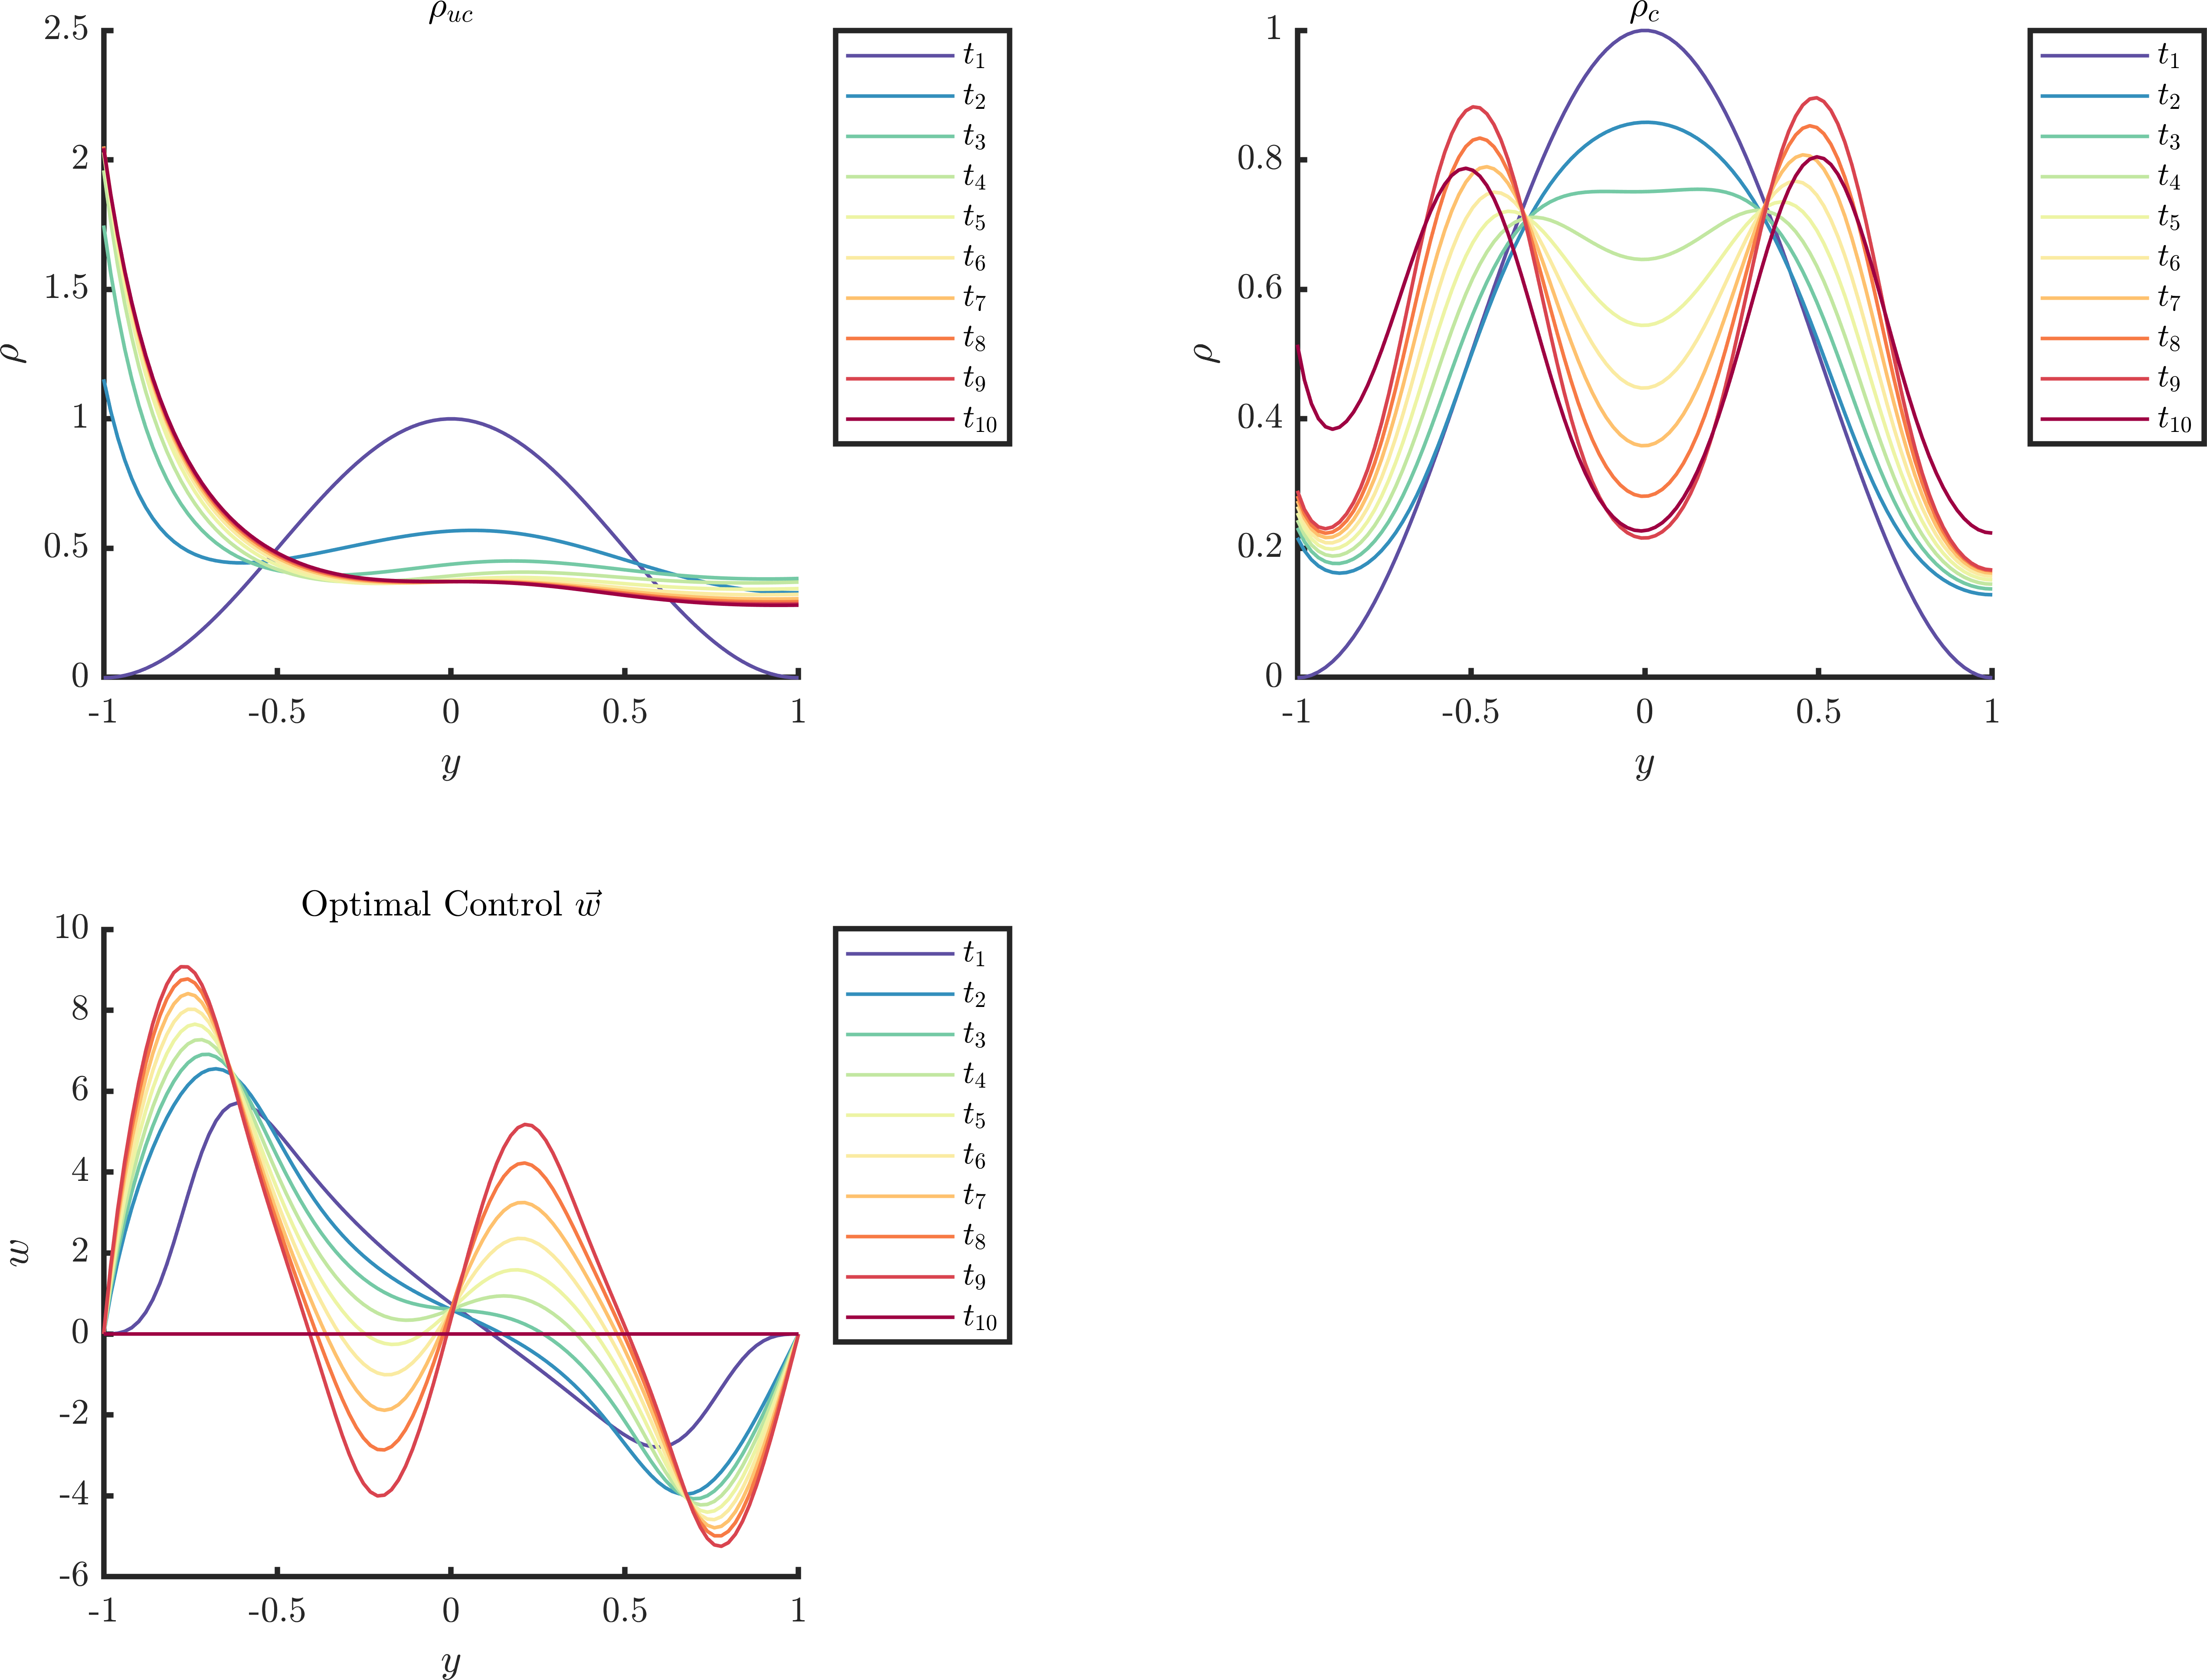
\includegraphics[scale=0.055]{V21.png}
	\caption{$V_{2}$, $\kappa = -1$} 
	\label{F3}
\end{figure}
\begin{figure}[h]
	\centering
	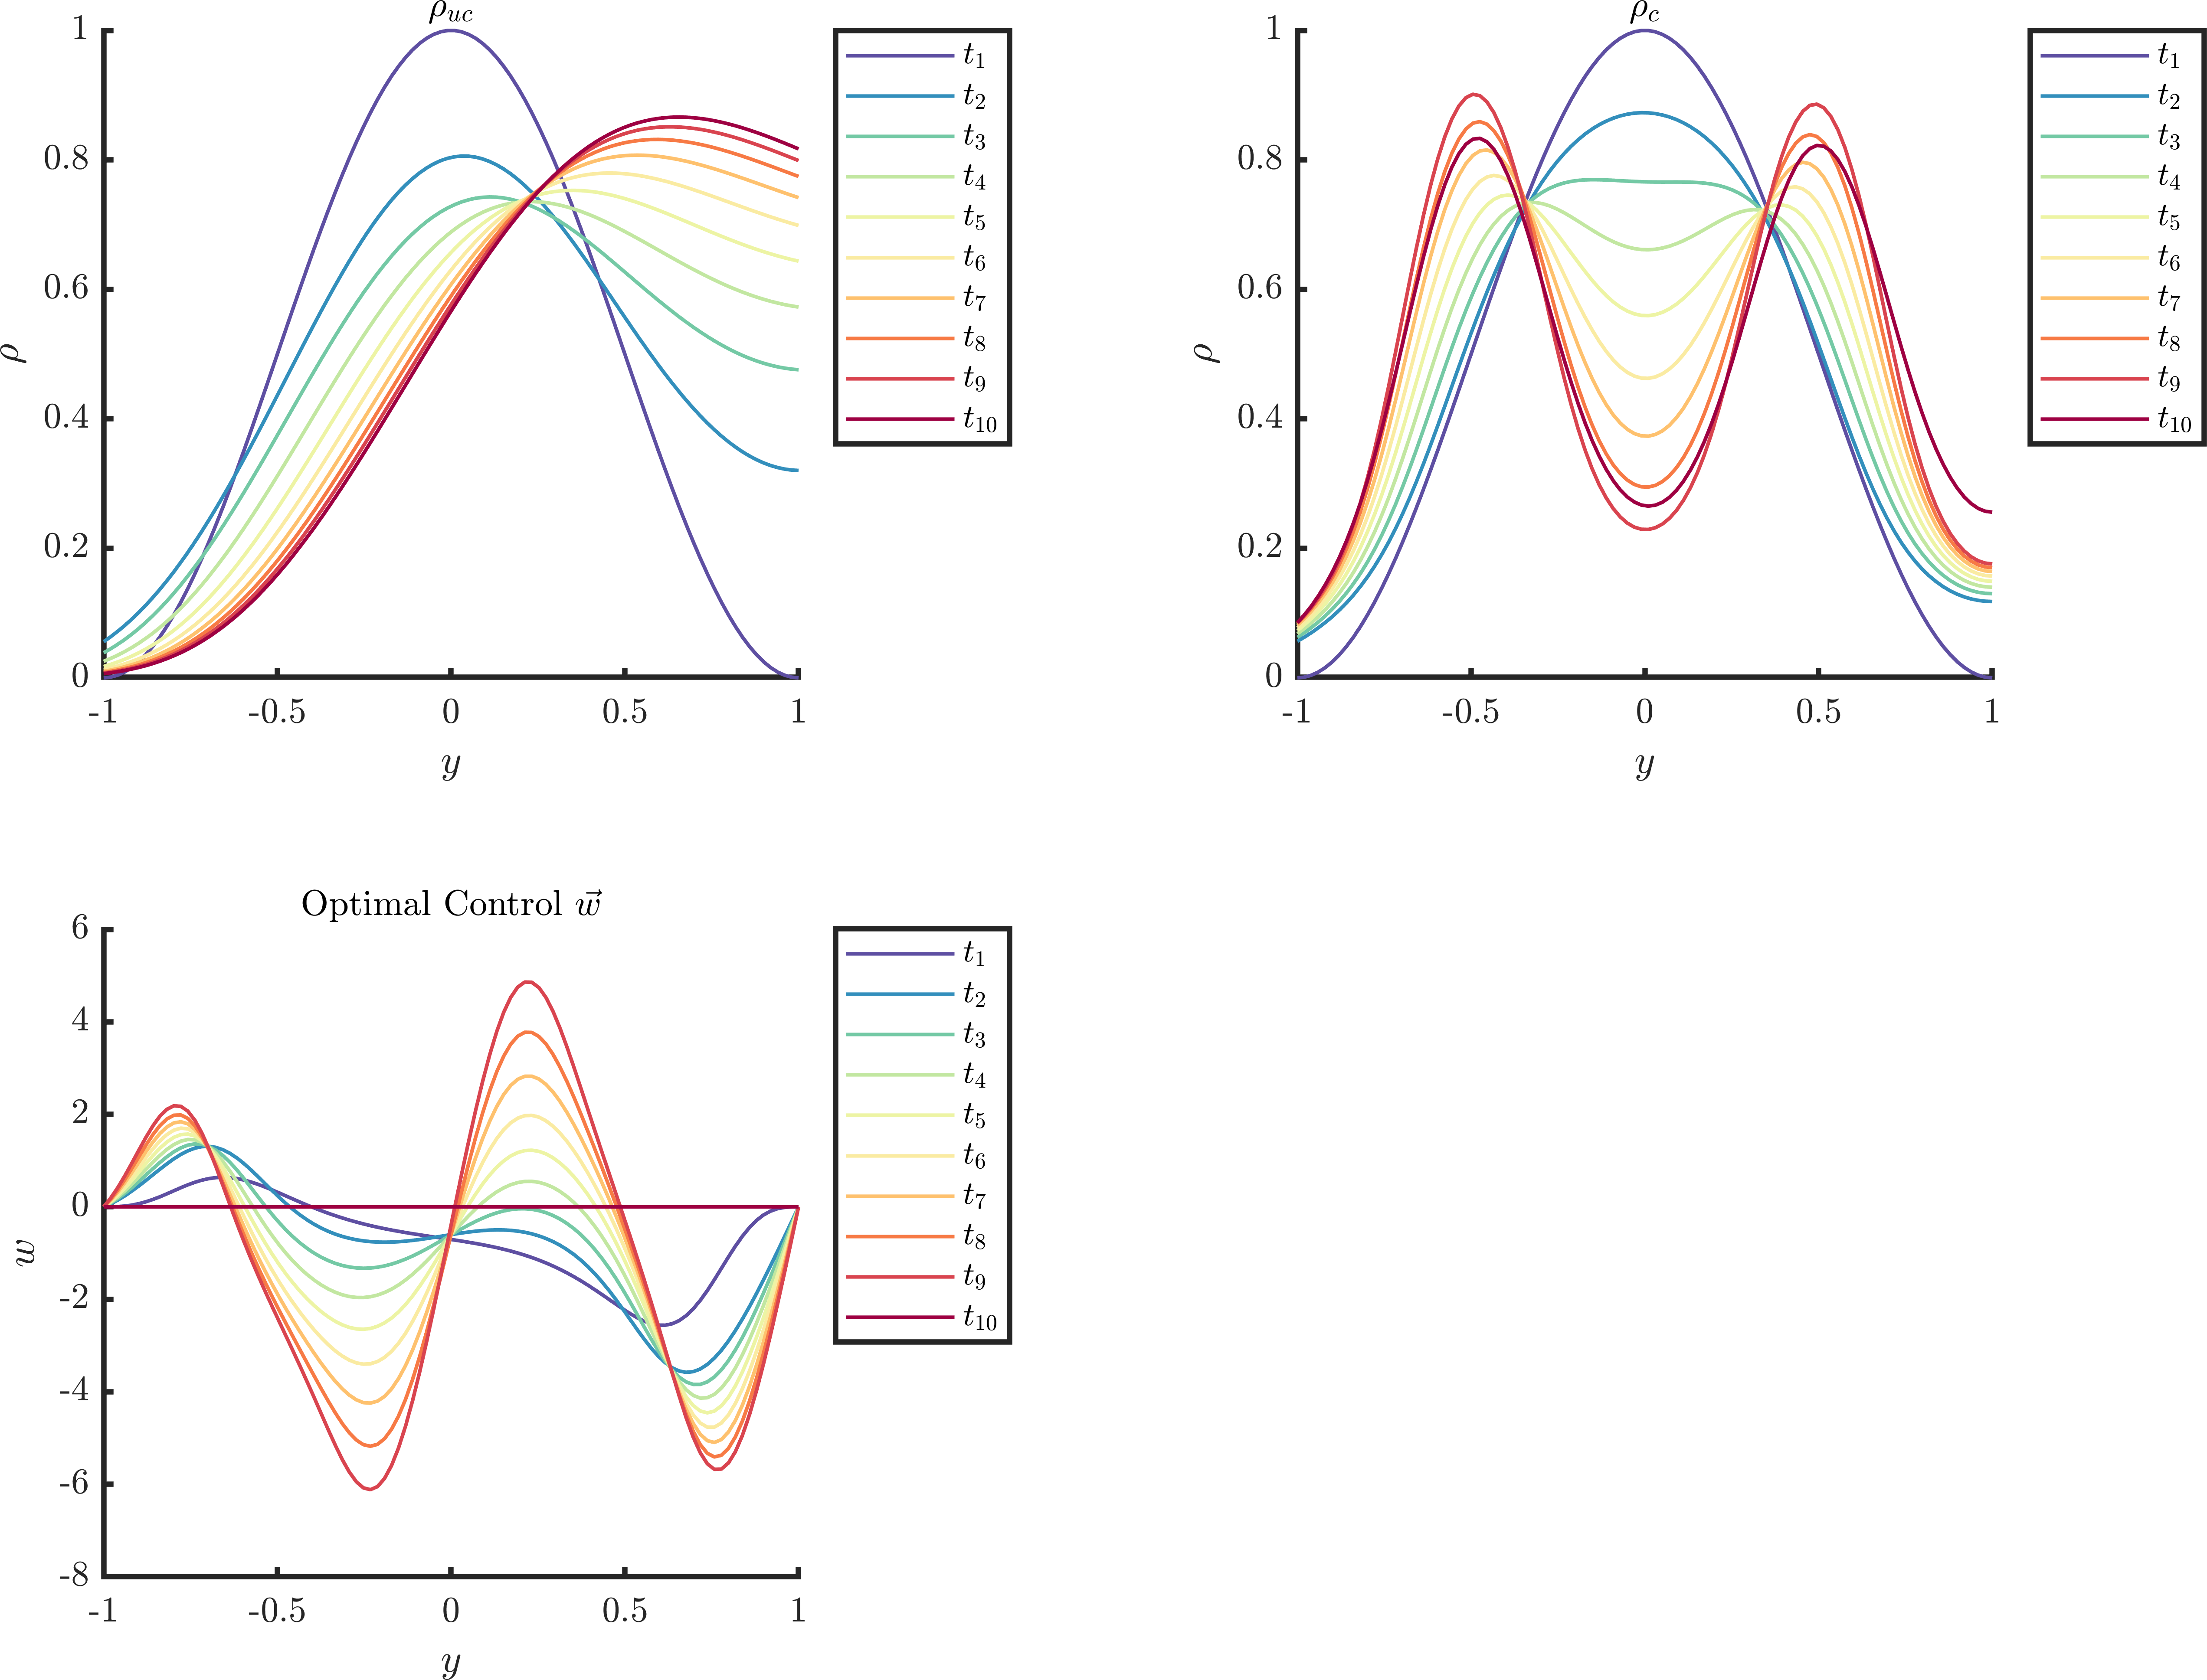
\includegraphics[scale=0.055]{V2p1.png}
	\caption{$V_{2}$, $\kappa = 1$} 
	\label{F3a}
\end{figure}



\end{document}